\documentclass[11pt,a4paper]{article}

\usepackage[T1]{fontenc}
\usepackage{lmodern}
\usepackage{microtype}
\usepackage[margin=24mm]{geometry}
\usepackage{graphicx}
\usepackage{booktabs}
\usepackage{amsmath}
\usepackage{siunitx}
\usepackage{xcolor}
\usepackage{hyperref}
\usepackage{cleveref}
\usepackage{caption}
\usepackage{subcaption}
\usepackage{float}
\usepackage{tikz}
\usetikzlibrary{arrows.meta,positioning,fit,calc}

\definecolor{gybeblue}{HTML}{126E82}
\definecolor{gybeorange}{HTML}{E67E22}
\definecolor{gybered}{HTML}{C0392B}
\hypersetup{
  colorlinks=true,
  linkcolor=gybeblue,
  urlcolor=gybeblue,
  citecolor=gybeblue,
  pdftitle={Reliable Offline Tracking for Long-Shot Windsurfing Video}
}

\graphicspath{{figures/}{../}{../../frontend/public/}}

\title{Reliable Offline Tracking for Long-Shot Windsurfing Video\\
\large Domain-specific pose, appearance, and global association}
\author{GybeLock / Windsurf Analysis}
\date{\today}

\begin{document}
\maketitle

\begin{abstract}
This report describes the engineering decisions behind a system that turns long-shot,
shore-recorded windsurfing footage into identity-consistent rider tracks and stable
focused views. The central challenge is not object count but error tolerance: a single
identity switch can contaminate the extracted video of a rider. Large camera pans,
small targets, prolonged co-visibility, and occlusions make generic online tracking a
poor fit. We therefore combine a domain-specific two-keypoint pose model, sail-color
appearance descriptors, camera-compensated motion, and offline global tracklet linking.
\end{abstract}

\section{Problem Definition and Operating Regime}
\label{sec:problem}

\subsection{The useful output is an identity-consistent video}

The input is long-shot windsurfing footage recorded from shore.  A typical scene
contains only a handful of surfers, so detection density is modest compared with
crowded pedestrian tracking.  The difficulty lies elsewhere: the subjects are small,
several sails can remain close or overlap for extended periods, and a rider may be
partly or fully occluded before reappearing.  Meanwhile, the operator follows the
action with large pans---about \SI{90}{\degree} in demanding examples, and sometimes
more.  Almost every background feature then moves in image coordinates, while the
visible background itself changes over the course of the shot.

\begin{figure}[t]
  \centering
  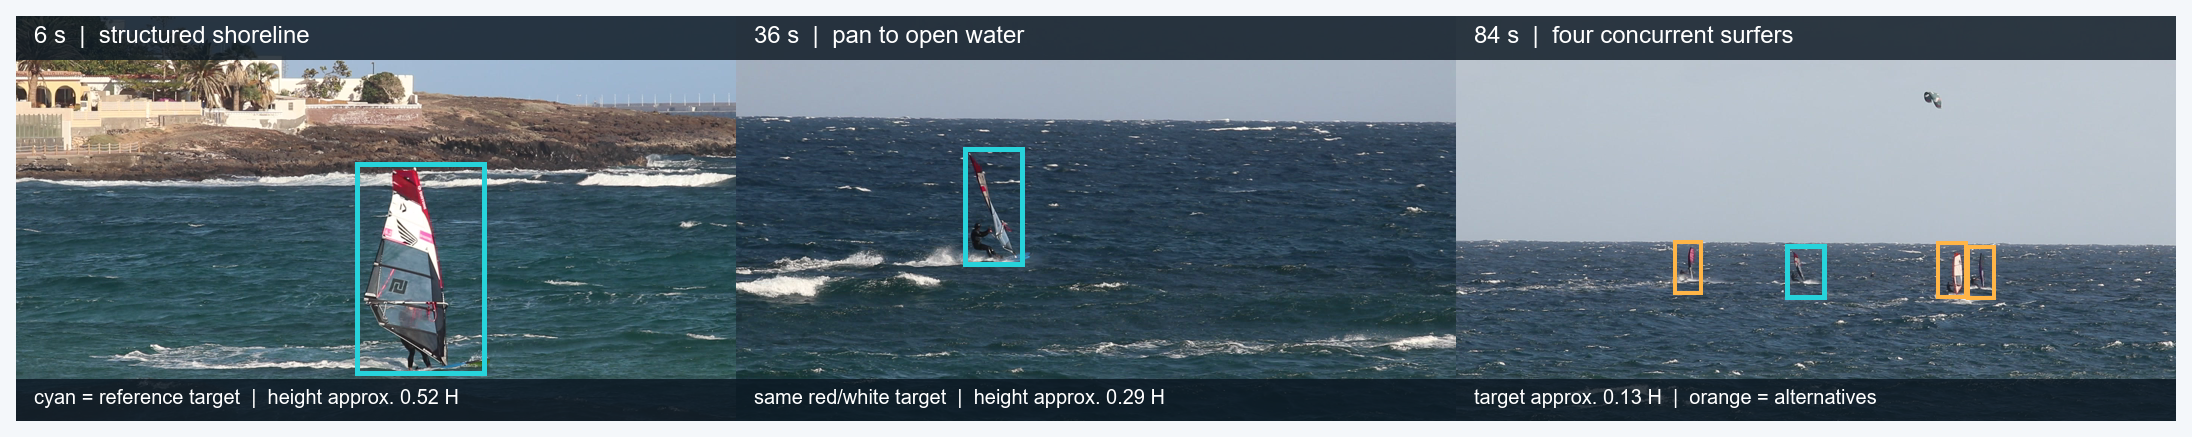
\includegraphics[width=\linewidth]{problem-camera-pan-scale-candidates.png}
  \caption{Representative frames from one project sequence at 6, 36, and
  \SI{84}{\second}.  The cyan annotation follows the same red-and-white sail as
  the camera moves from shoreline to open water; its image height changes from
  approximately $0.52H$ to $0.13H$.  At \SI{84}{\second}, three other surfers
  (orange) are visible alongside it as plausible association candidates.  The
  composite illustrates changing background, scale variation, and identity
  ambiguity within one shot.}
  \label{fig:problem-operating-regime}
\end{figure}

The desired result is not merely a plausible bounding box in most frames.  It is a
separate, continuous trajectory for each physical surfer, suitable for extracting a
focused rider video.  If a track changes identity once, the resulting video jumps to
another rider and can no longer serve its purpose.  Identity consistency is therefore
the primary objective; smooth localization and high detection recall matter only
after that constraint is met.

We consequently treat association errors asymmetrically.  A missed link produces two
fragments that can be inspected or joined later.  A false link contaminates an
otherwise valid trajectory and may invalidate the complete extracted sequence.  In
ambiguous cases, fragmentation or abstention is preferable to an unjustified merge.
This is a design requirement---effectively zero tolerance for identity switches---not
a claim that the present system achieves perfect tracking on arbitrary footage.

\subsection{Why ordinary online tracking is a poor fit}

General-purpose multi-object trackers commonly process frames causally: they predict
each active track into the next frame, assign the current detections, and carry that
decision forward.  This is attractive for real-time operation, but it commits at the
moment evidence is weakest.  During a crossing or occlusion, two continuations can be
equally plausible from past motion alone; evidence that appears several seconds later
cannot undo an early identity switch reliably.

Raw image-space motion is also a misleading cue in this regime.  During a pan, a
stationary background point and every surfer receive a large common displacement.
The residual motion of an individual surfer may be much smaller than this camera
component.  Association therefore depends on estimating global camera motion and
applying it to the motion model before comparing a prediction with a detection.  The
production pipeline makes this coupling explicit: it estimates masked frame-to-frame
transforms while excluding detected surfers, then passes those transforms to both the
greedy tracklet builder and the global linker
(\texttt{video\_processing/main\_tracking.py}).

There is no real-time requirement for the final analysis: the complete recording is
available before a focused video is generated.  The system uses that freedom in two
stages.  A conservative causal pass accepts only clear local matches and leaves
ambiguous observations as separate tracklets.  An offline integer programming pass
then evaluates feasible links between those tracklets jointly, using evidence on both
sides of a gap.  Its graph includes the option to begin or end a trajectory instead of
forcing a link, and can discard very short suspected false-positive fragments
in the production tracking implementation.  Thus future evidence informs
association without weakening the conservative local decisions that protect track
purity.

The problem is therefore narrower than general multi-object tracking, but its loss
function is harsher: few objects, difficult camera motion, long periods of ambiguity,
and an output that is useful only while identity remains intact.  The remainder of
this report explains how pose, sail-specific appearance, camera compensation, and
offline global association were chosen around that operating regime.

\section{Pose as a Stable Virtual Camera Signal}
\label{sec:pose}

Tracking answers \emph{which} surfer is present in each frame, but a useful focused
view also needs to decide where to place the virtual camera and how tightly to crop.
A detector bounding box is a poor control signal for this purpose.  A windsurf rig
is articulated, strongly anisotropic, and continually rotates with respect to the
camera.  Its axis-aligned box can therefore change width, height, and centre even
when the rider has moved little and remains at approximately the same distance.
Using the box centre and height directly makes the crop drift across the subject and
causes visible zoom pumping.

\subsection{Two semantic points instead of a generic human pose}

The production detector is a YOLO pose model supervised for one class and two
domain-specific keypoints: the boom--mast junction and the mast tip.  These points
were chosen for the rendering geometry rather than to describe the complete human
body.  The boom--mast junction gives a repeatable reference near the rider and sail,
while the distance from that junction to the mast tip provides a rig-relative scale cue
that is substantially less sensitive than an axis-aligned box height to in-plane
rotation.

The labels build on the manually reviewed detection boxes.  A dedicated annotation
tool presents an enlarged crop for each box, permits either keypoint to be marked as
not visible, and writes two-keypoint YOLO pose labels.  The checked-in pose project
contains 1,123 manually labelled training images and 56 validation images.  The
workflow also supports conservative pseudo-labelling: a prediction is accepted only
after matching it to an existing box and applying detection, overlap, keypoint
confidence, and spatial plausibility gates; pseudo-labels remain separate from manual
labels and are included in training only when requested.  Finally, a hard-window
miner runs the complete local pipeline and ranks short intervals by keypoint jitter
relative to the rendered anchor.  This directs subsequent review towards failures
that are visually disruptive in the final crop, rather than towards another uniform
sample of easy frames.

\subsection{From keypoints to crop centre}

For a detection with bounding box top $y_1$, height $h$, and centre
$(c_x,c_y)$, the fallback anchor is
\begin{equation}
  \mathbf{a}_{\mathrm{box}} = (c_x,\; y_1 + 0.6h).
  \label{eq:pose-box-anchor}
\end{equation}
Placing it below the geometric box centre is a deliberate bias towards the rider and
board rather than the empty upper part of a tall sail box.  When the boom--mast
junction $\mathbf{b}=(b_x,b_y)$ is visible, the implementation first constructs a
low-noise proxy for the mast tip, $\tilde{\mathbf{t}}=(b_x,y_1)$, and places the
semantic anchor at
\begin{equation}
  \mathbf{a}_{\mathrm{pose}}
    = 0.15\tilde{\mathbf{t}} + 0.85\mathbf{b}.
  \label{eq:pose-semantic-anchor}
\end{equation}
Thus the crop is anchored slightly above the boom junction.  The measured mast-tip
coordinate is intentionally not used for position: its larger lever arm would turn
localization noise into unnecessary crop motion.  It remains valuable for scale.

\begin{figure}[t]
  \centering
  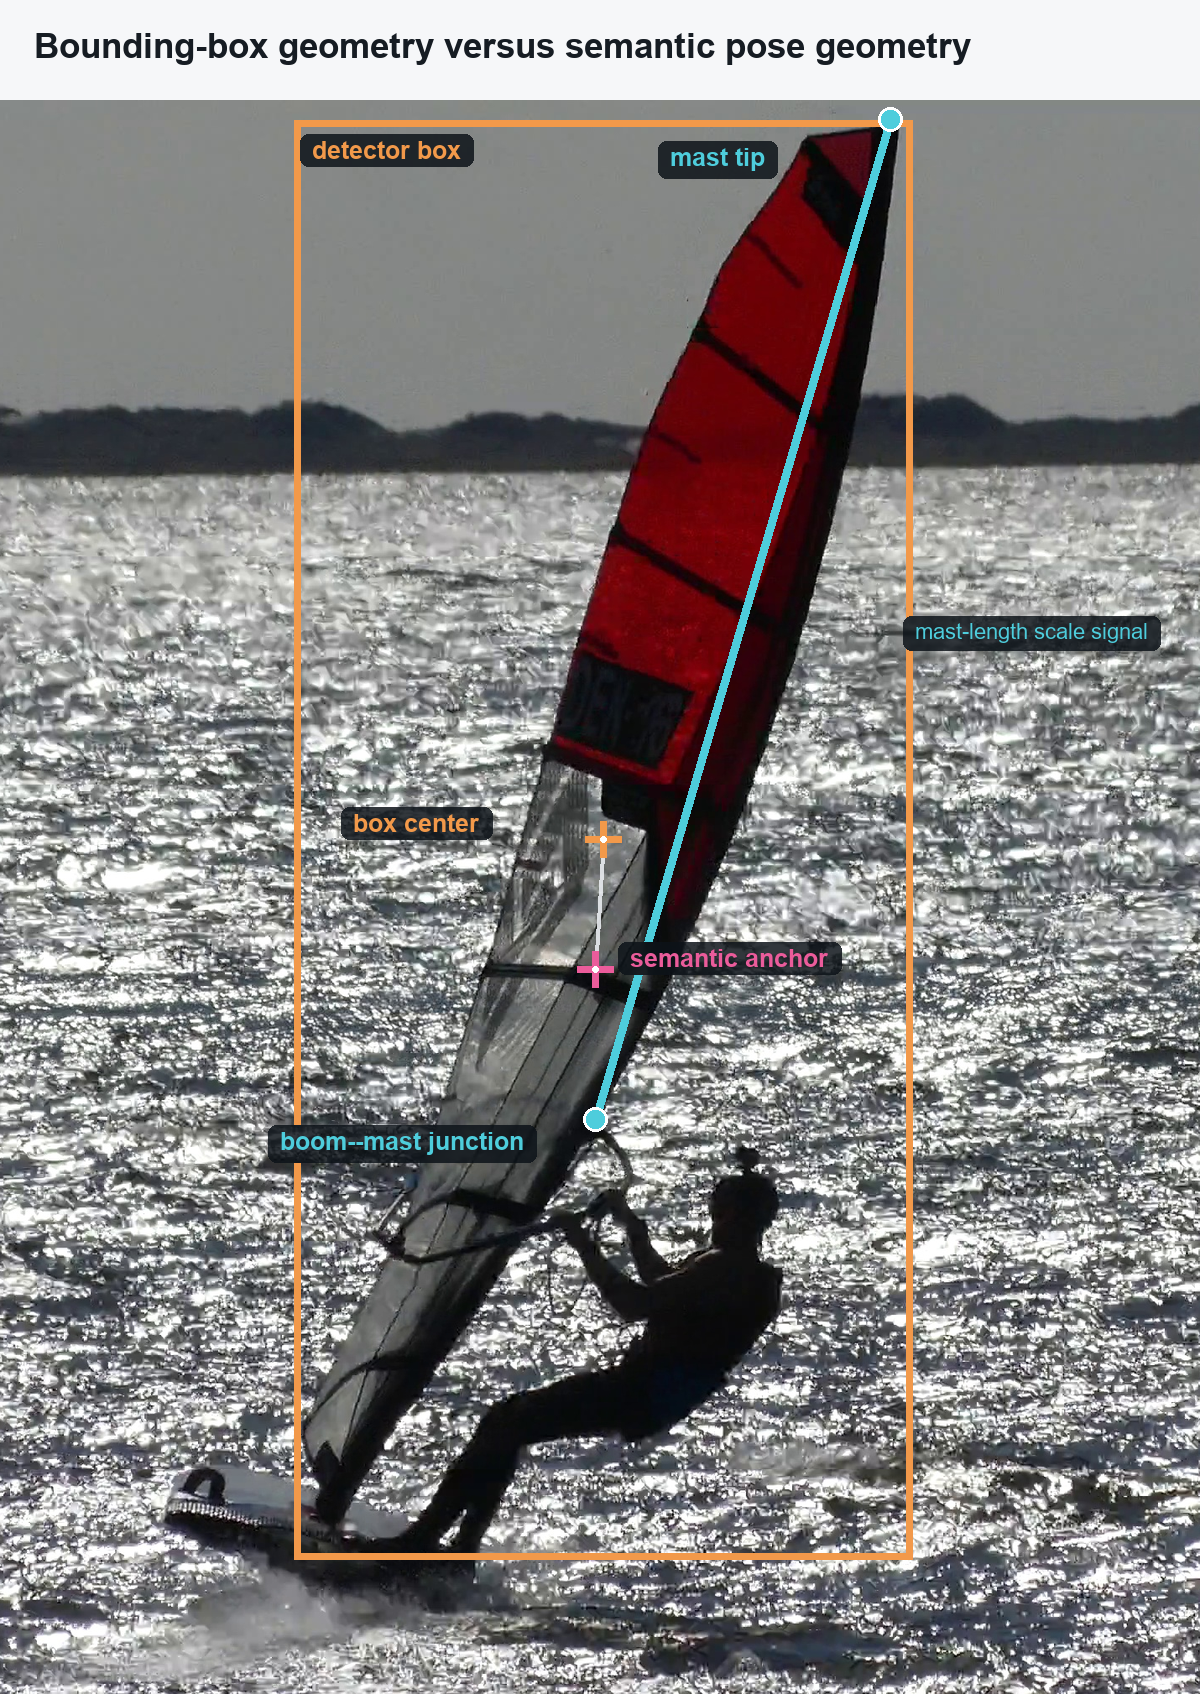
\includegraphics[width=0.58\linewidth]{pose-anchor-geometry.png}
  \caption{Pose-derived virtual-camera geometry on a representative labelled
  frame.  The detector box and its centre (orange) describe image extent.  The
  boom--mast junction and mast tip (cyan) instead provide a rider-relative anchor
  (magenta) and a rig-relative scale cue.  Production rendering smooths these
  signals over time and falls back to box geometry when keypoints are unavailable.}
  \label{fig:pose-anchor-geometry}
\end{figure}

Small detections do not contain enough pixels for equally reliable keypoint
localization.  The final unsmoothed anchor therefore blends
$\mathbf{a}_{\mathrm{pose}}$ with $\mathbf{a}_{\mathrm{box}}$ according to the
shorter box dimension.  The pose weight rises linearly from zero at 45 pixels to one
at 55 pixels.  A keypoint is considered visible at confidence 0.15 or greater; below
that threshold, the box fallback is used.

Missing observations are handled as transitions, not abrupt mode switches.  Gaps of
up to five frames between visible boom keypoints are interpolated directly between
semantic anchors.  Across longer gaps, the anchor eases from the last semantic point
to the per-frame box fallback and eases back when a reliable keypoint returns.
Leading and trailing missing spans receive analogous fallback or short hold
behaviour.  A final five-frame robust weighted mean suppresses isolated jumps while
giving the current frame the largest weight; Huber reweighting limits the influence
of spatial outliers.  This processing operates on the dense tracks produced by the
tracking post-processor, so every frame in a track receives an anchor even when its
detection was interpolated.

\subsection{A scale tied to the rig}

When both keypoints are visible, the scale signal is the Euclidean length
$\ell=\lVert\mathbf{b}-\mathbf{t}\rVert_2$ of the observed boom-to-tip mast
segment.  Short missing spans are interpolated and the last valid value is held for
up to five frames; otherwise the vertical distance from the current anchor to the
box top supplies a fallback.  A centred moving mean with radius 15 frames smooths
this length signal.  The requested crop height in pixels is then
\begin{equation}
  C = \max\!\left(\frac{\bar{\ell}}{0.75},
                  \frac{h}{0.9}, 1\right),
  \qquad s = \operatorname{clip}\!\left(\frac{C}{H},10^{-6},1\right),
  \label{eq:pose-scale}
\end{equation}
where $H$ is the source-video height.  The first term aims to make the semantic mast
segment occupy 75\% of the output height; the second prevents the detected box from
being cropped more tightly than a 90\% fill.  Taking the maximum preserves context
when either signal calls for a wider view.

The resulting normalized anchor and scale are stored with every renderable
detection and consumed directly by the focused player.  They stabilize the
\emph{composition} of an individual rider: which semantic point stays near the
centre and how large the rig appears.  This is distinct from global camera-motion
compensation.  The latter estimates frame-to-frame background transforms (while
masking detected surfers), supports motion-based association, and supplies an
optional stabilized overview.  It does not replace the pose-derived virtual camera;
a globally stabilized frame can still contain a rotating rig whose bounding box
centre and dimensions fluctuate.

\section{Offline Identity Association}
\label{sec:tracking}

The tracker converts detections into high-purity local fragments and then into
globally consistent paths.  The same camera-motion estimates support both stages.

\begin{figure}[t]
  \centering
  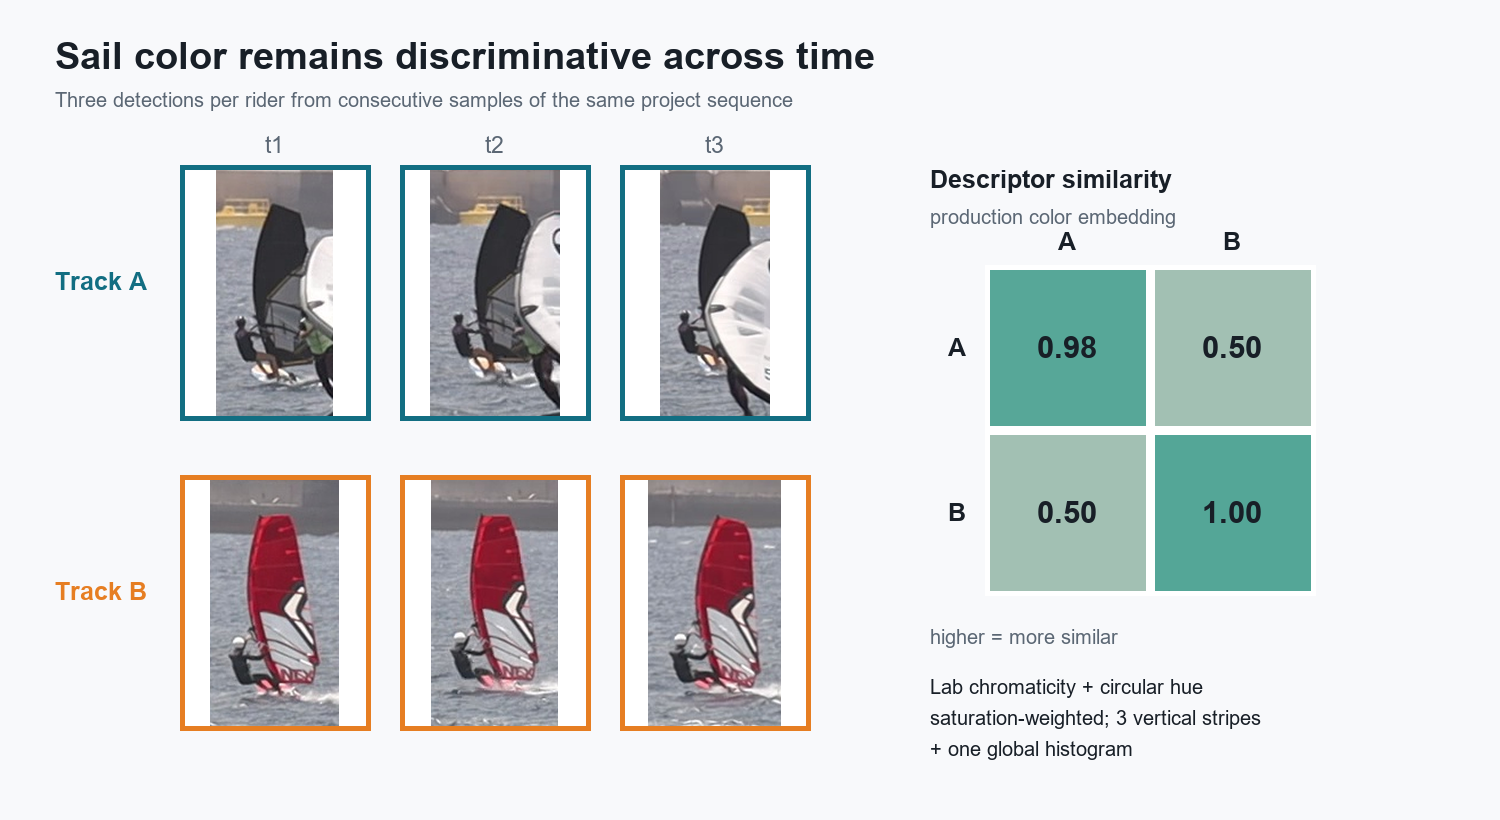
\includegraphics[width=\linewidth]{tracking-sail-color-similarity.png}
  \caption{Production color descriptor on consecutive crops of two sails.  Repeated
  observations score highly, while cross-sail matches reach the lower bound.  The
  hand-selected example explains the cue rather than measuring it.}
  \label{fig:tracking-sail-color}
\end{figure}

\subsection{Foreground-masked sail appearance}

Windsurfing sails are large, saturated, and often visually distinctive even when the
rider occupies only a few pixels.  For each detection crop we build a descriptor from
a joint histogram of the chromatic Lab channels $(a,b)$, a circular hue histogram,
and a lower-weight luminance histogram.  Saturation weighting emphasizes colored sail
panels over gray water, spray, and haze.  Three vertical bands preserve coarse color
layout, and a fourth block represents the complete crop.  Each block is L1-normalized
and square-root mapped before the concatenated vector is L2-normalized, yielding a
bounded Hellinger-style distance.

\Cref{fig:tracking-sail-color} illustrates the descriptor response on two visually
distinct sails.

The descriptor first removes likely background using a border-derived Lab model.  A
gradient gate identifies low-texture pixels consistent with that model, and only
candidate background components connected to the crop border are removed.  After
morphological cleanup, only the largest remaining foreground component is retained;
a minimum-mask fallback avoids empty descriptors.  This foreground mask is important: an earlier inactive code
path used a fixed center rectangle, allowing water and overlapping sails to dilute
the intended cue.

\Cref{fig:tracking-offline-association} contrasts the locally ambiguous online view
with the later fragment evidence available to the offline optimizer.

\begin{figure*}[t]
  \centering
  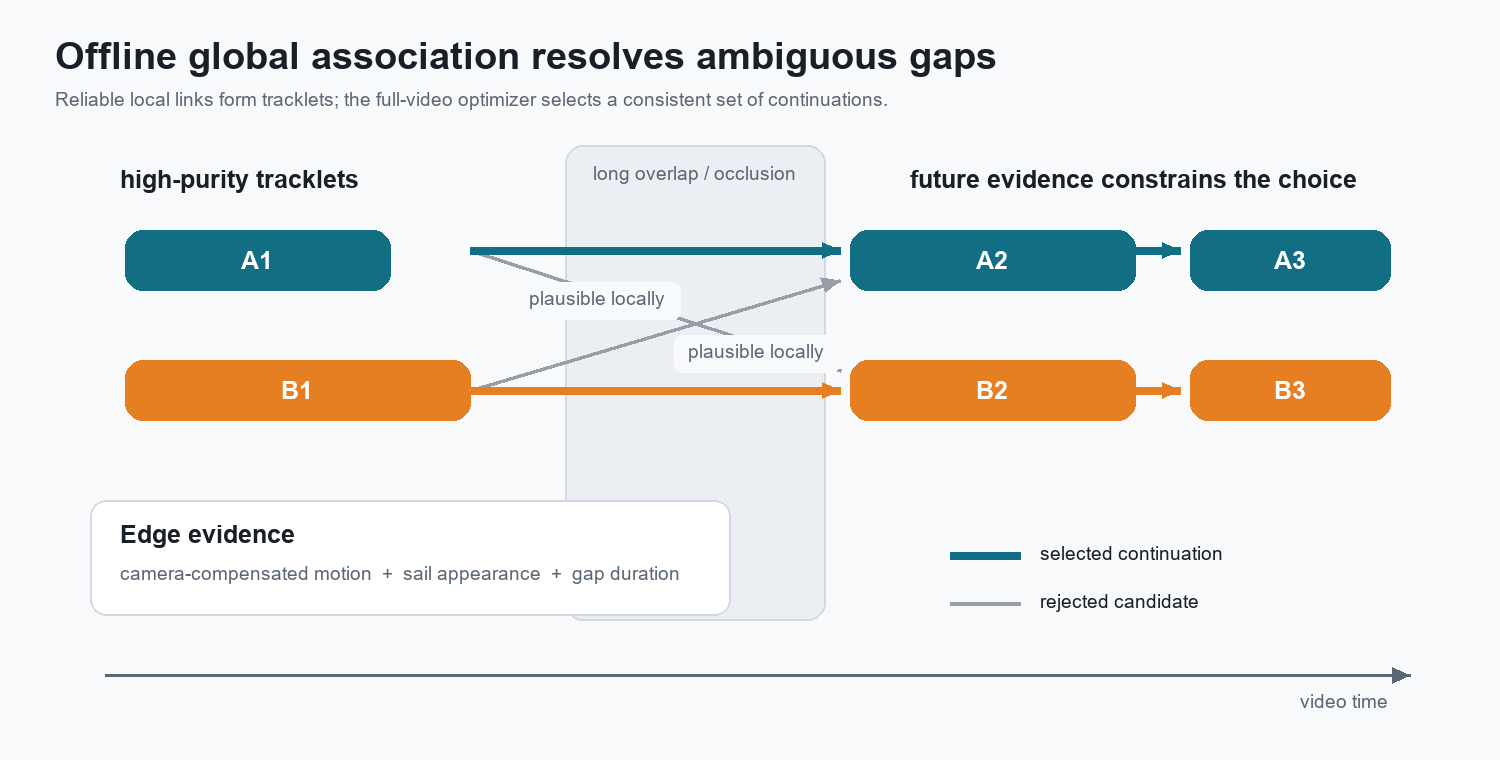
\includegraphics[width=0.82\textwidth]{tracking-offline-global-association.png}
  \caption{Future fragment evidence supports global tracklet association.  Later
  stable observations distinguish locally ambiguous successors; the optimizer then
  chooses a compatible pairing jointly.  Start, end, discard, and gap costs are
  omitted from the conceptual diagram.}
  \label{fig:tracking-offline-association}
\end{figure*}

For a tracklet, all observation embeddings are averaged into a whole-fragment
prototype.  This replaced endpoint-biased exponential averages, which emphasized the
last crop of the earlier fragment and first crop of the later fragment---exactly the
frames most likely to contain both sails during a crossing.  Given descriptor distance $d$, the
current heuristic match score is
\begin{equation}
 \begin{aligned}
 \epsilon&=10^{-6},\\
 S_a&=\operatorname{clip}_{[\epsilon,\,1-\epsilon]}(1-\gamma_a d),
 &\gamma_a&=11.63.
 \end{aligned}
 \label{eq:appearance}
\end{equation}
It is a tuned similarity score, not a calibrated posterior probability; the graph
uses $C^{\mathrm{appearance}}=-\log S_a$.  The coefficient $\gamma_a$ was tuned on the
development set.  The numerical margin $\epsilon$ keeps the logarithm well defined.

\subsection{Conservative local tracklets}

Each detection initially forms a singleton.  A greedy preprocessor advances a
constant-velocity Kalman state~\cite{kalman} through the estimated frame-to-frame
camera transforms and compares the prediction with current detections.  Strict links
require both motion and appearance evidence; looser links are accepted only when they
are unique.  Duplicate proposals, competing successors, or multiple plausible
candidates remain separate.  The local stage therefore sacrifices completeness to
preserve fragment purity.

This behavior is deliberate.  In the evaluation reconstruction, 598 of 601
preprocessor fragments are pure with respect to retained gold identities.  The
dominant catastrophic error is introduced later when two pure fragments are linked
incorrectly, which makes the offline edge decision the appropriate place for
additional safeguards.

\subsection{Candidate graph}

For non-overlapping fragments $T_i$ and $T_j$, a directed candidate $i\rightarrow j$
is created only when the gap is at most three seconds.  A Kalman state fitted to all
detections of $T_i$ is propagated to the first observations of $T_j$, applying global
camera transforms at every intervening frame.  Unlike the earlier production call,
the gate uses the complete measurement $(c_x,c_y,w,h)$ rather than discarding width
and height.

Every candidate receives
\begin{equation}
 \begin{aligned}
 C_{ij}={}&w_m C^{\mathrm{motion}}_{ij}
       +w_a C^{\mathrm{appearance}}_{ij}\\
       &+w_g C^{\mathrm{gap}}_{ij},\\
 C^{\mathrm{gap}}_{ij}={}&-\Delta f_{ij}\log p_{\mathrm{miss}}.
 \end{aligned}
 \label{eq:edge-cost}
\end{equation}
For each of the first two observations of $T_j$, the predicted Kalman state gives
squared Mahalanobis distance $d^2$ over $(c_x,c_y,w,h)$.  Motion cost is the mean
negative log chi-square survival score, $-\log\Pr(\chi^2_4\geq d^2)$; appearance uses
the whole-fragment prototypes; and the gap term increases with the number of missing
frames.

The graph now applies absolute plausibility vetoes before optimization.  Edges are
removed when motion cost exceeds 8, or when endpoint box area or aspect ratio changes
by more than a factor of three.  The Kalman filter already models size; the explicit
ratios supplement it with an interpretable discontinuity bound.  These rules implement
abstention at the evidence boundary.  They are necessary because a central fragment's
start and end penalties can otherwise make even poor finite evidence cheaper than
leaving two trajectories separate.

\subsection{Global path optimization}

Binary variables represent starting or ending a path at each fragment, selecting a
candidate edge, or discarding an eligible short fragment.  Each retained fragment has
exactly one incoming choice and one outgoing choice, so selected links form disjoint,
time-ordered paths.  Start and end costs are reduced near image borders, where a
surfer entering or leaving the field of view is more plausible.  An edge that costs
more than ending $T_i$ and starting $T_j$ independently is dominated and removed; the
remaining outgoing degree is bounded before solving the integer program.

The method is offline in a precise sense: it compares stable fragments on both sides
of a gap and chooses all compatible continuations jointly.  It does not infer through
arbitrarily long absence.  Gaps beyond the horizon remain fragmented, and ambiguous
evidence should do the same.

\subsection{Dense trajectories}

Linked detections remain sparse.  The post-processor removes tracks that are too short
or sparsely observed, performs a forward camera-compensated Kalman pass and backward
Rauch--Tung--Striebel smoothing~\cite{rts}, and interpolates internal gaps.  The dense
trajectory records whether each observation was detected or synthesized, then feeds
the rider-relative stabilization stage.

\section{Evaluation}
\label{sec:evaluation}

We evaluate identity association on 21 manually curated development videos.  The
benchmark fixes the universe of 41,079 saved, non-interpolated detections and gives
every method the same bounding boxes.  Of these, 41,004 belong to retained surfer
identities and 75 are annotated for rejection.  This deliberately isolates
association from detector recall: the results answer whether the available
observations were grouped correctly, not whether YOLO found every surfer.

The saved observations were selected during manual trajectory reconstruction and
their boxes were Rauch--Tung--Striebel smoothed afterwards.  The benchmark is
therefore conditional on gold-derived observations rather than an end-to-end MOT
test.  It is also an in-sample development-set evaluation: algorithm design was
informed by these videos, and the provenance of the original ILP parameter tuning is
not fully recorded.  We report the results as engineering evidence and failure
analysis, not as a held-out leaderboard.

\subsection{Metrics}

For retained detections, pairwise precision and recall compare every unordered pair.
A pair is positive when both observations have the same annotated identity:

\begin{align}
  P_{\mathrm{pair}} &=
    \frac{\text{correct same-identity pairs}}
         {\text{all pairs joined by the tracker}}, \\
  R_{\mathrm{pair}} &=
    \frac{\text{correct same-identity pairs}}
         {\text{all annotated same-identity pairs}}.
\end{align}

False merges reduce precision and fragmentation reduces recall.  Missing outputs are
treated as singleton predictions rather than being silently omitted.  Micro scores
pool all pairs and consequently weight long identities quadratically; macro scores
average per-video values.  We additionally report contaminated predicted tracks,
which contain more than one gold identity; fragmentation excess, the number of
predicted pieces beyond one per gold identity; and exact videos, whose complete
partition matches the annotation up to track-label permutation.  These absolute
counts matter because a high aggregate F1 can conceal one application-breaking
identity switch.

\subsection{Fixed-observation comparison}

\Cref{tab:association-benchmark} compares the production pipeline with OC-SORT and
BoT-SORT.  OC-SORT receives the fixed detections directly.  BoT-SORT uses its ECC
camera compensation but no pedestrian-specific ReID network.  The production method
reruns conservative preprocessing, masked video stabilization, and offline ILP
association.  Its sail descriptor uses border-derived foreground masking and a
whole-fragment appearance prototype; motion gating evaluates centre, width, and
height; and implausible motion, area, or aspect-ratio transitions are excluded before
optimization.

\begin{table*}[t]
  \centering
  \small
  \caption{Fixed-observation identity-association results on 21 development videos.
  ``Contam.'' counts predicted tracks containing more than one gold identity.}
  \label{tab:association-benchmark}
  \begin{tabular}{lrrrrrrr}
    \toprule
    Method & Coverage & Pair P & Pair R & Pair F1 & Macro F1 & Contam. & Frag. excess \\
    \midrule
    OC-SORT & 0.981 & \textbf{0.985} & 0.662 & 0.792 & 0.857 & 9/165 & 845 \\
    BoT-SORT, no ReID & 0.996 & 0.920 & 0.752 & 0.828 & 0.858 & 16/142 & 244 \\
    Production offline ILP & \textbf{0.999} & 0.957 & \textbf{0.918} & \textbf{0.937} & \textbf{0.970} & 9/95 & \textbf{42} \\
    \bottomrule
  \end{tabular}
\end{table*}

The production system gives the strongest overall association score and reduces
fragmentation by a factor of approximately six relative to BoT-SORT and by a factor
of twenty relative to OC-SORT.  Eleven of 21 videos are exact, compared with
four for BoT-SORT and one for OC-SORT.  OC-SORT attains the highest pairwise precision
by remaining highly conservative, but its 845 excess fragments do not provide the
continuous identity track required by the application.  The production result is a
more useful operating point for this dataset, but its nine contaminated tracks mean
that it still does not satisfy the nominal zero-false-merge requirement.

Runtime is included only as an operational diagnostic.  On the evaluation machine,
OC-SORT took 9.0 seconds, BoT-SORT 497.7 seconds, and the production association path
402.3 seconds.  The workloads are not identical: OC-SORT needs no video decode,
BoT-SORT includes decode and ECC, and production includes masked stabilization but
excludes the initial crop-embedding extraction.

\subsection{Safeguard ablation}

The initial production reconstruction exposed a concentrated false-link problem.
Preprocessor fragments were almost always identity-pure, but the ILP sometimes joined
two pure fragments from different surfers.  Many of the unexpected short-gap errors
occurred at crossings, where the endpoint crops contained both sails.  The previous
appearance model emphasized precisely those boundary frames, the color descriptor's
intended foreground mask was bypassed by an early return, and the ILP requested a
position-only projection from a Kalman model that already represented width and
height.

\Cref{tab:safeguard-ablation} records two staged revisions.  Because several changes
are bundled in the first stage, this is a system ablation rather than a claim that any
single component produced the full difference.  Foreground masking, whole-fragment
appearance aggregation, and four-dimensional motion evaluation raise micro F1 from
0.893 to 0.928.  Adding conservative vetoes for motion NLL and threefold area or
aspect-ratio discontinuities raises precision further and halves contaminated tracks,
without increasing fragmentation.

\begin{table}[t]
  \centering
  \scriptsize
  \caption{Staged production-pipeline revision on the same development set.}
  \label{tab:safeguard-ablation}
  \begin{tabular}{@{}lrrrrr@{}}
    \toprule
    Stage & P & R & F1 & Cont. & Frag. \\
    \midrule
    Original & 0.907 & 0.880 & 0.893 & 20 & 48 \\
    + mask, mean, 4D & 0.939 & 0.917 & 0.928 & 17 & 44 \\
    + conservative vetoes & \textbf{0.957} & \textbf{0.918} & \textbf{0.937} & \textbf{9} & \textbf{42} \\
    \bottomrule
  \end{tabular}
\end{table}

The vetoes are not a second tracker layered on top of the Kalman filter.  The Kalman
state already contains centre, width, and height; the earlier ILP call discarded the
size dimensions.  The revised system uses the full four-dimensional Mahalanobis
evidence and additionally refuses links whose absolute evidence is implausible.  This
second step is necessary because the ILP's start and end penalties can otherwise make
even a very poor link cheaper than splitting two central fragments.

A manual audit found nine wrong selected fragment joins.  Unlike the removed
geometric failures, they concentrate at crossings, visually near-identical sails,
and crops containing both competitors.  Their implications and the unsuccessful
global-margin abstention experiment are discussed in \Cref{sec:discussion}.

\section{Delivering Frame-Accurate Results in the Browser}
\label{sec:player}

Tracking results are indexed by frame, so detections, transforms, pose anchors, and
annotations must refer to the image actually displayed. An ordinary HTML video
element exposes media time rather than stable frame identity, which is insufficient
for frame stepping, hit-testing, and inspection across an occlusion.

The WebCodecs path~\cite{webcodecs} discards packets with negative presentation
timestamps (PTS), then orders the remainder by PTS and packet sequence number. Position
in that list is the canonical zero-based frame index. Preview seeks from a preceding
keyframe and decodes forward, reusing a bounded cache for nearby frames. A result is
published only if it still belongs to the latest seek.

Export decodes independently, advances through the same packet-index convention, and
resynchronizes to the closest PTS if necessary. The recovered index selects the rider
track. Overview preview additionally reads the global stabilization transform, whereas
focused preview and export share the pose-anchor crop function. Decoded images and
output surfaces remain separate. This machinery is not a tracking contribution; it
makes the result inspectable and exportable without silently shifting an overlay or
crop to a neighboring frame.

\begin{figure}[t]
  \centering
  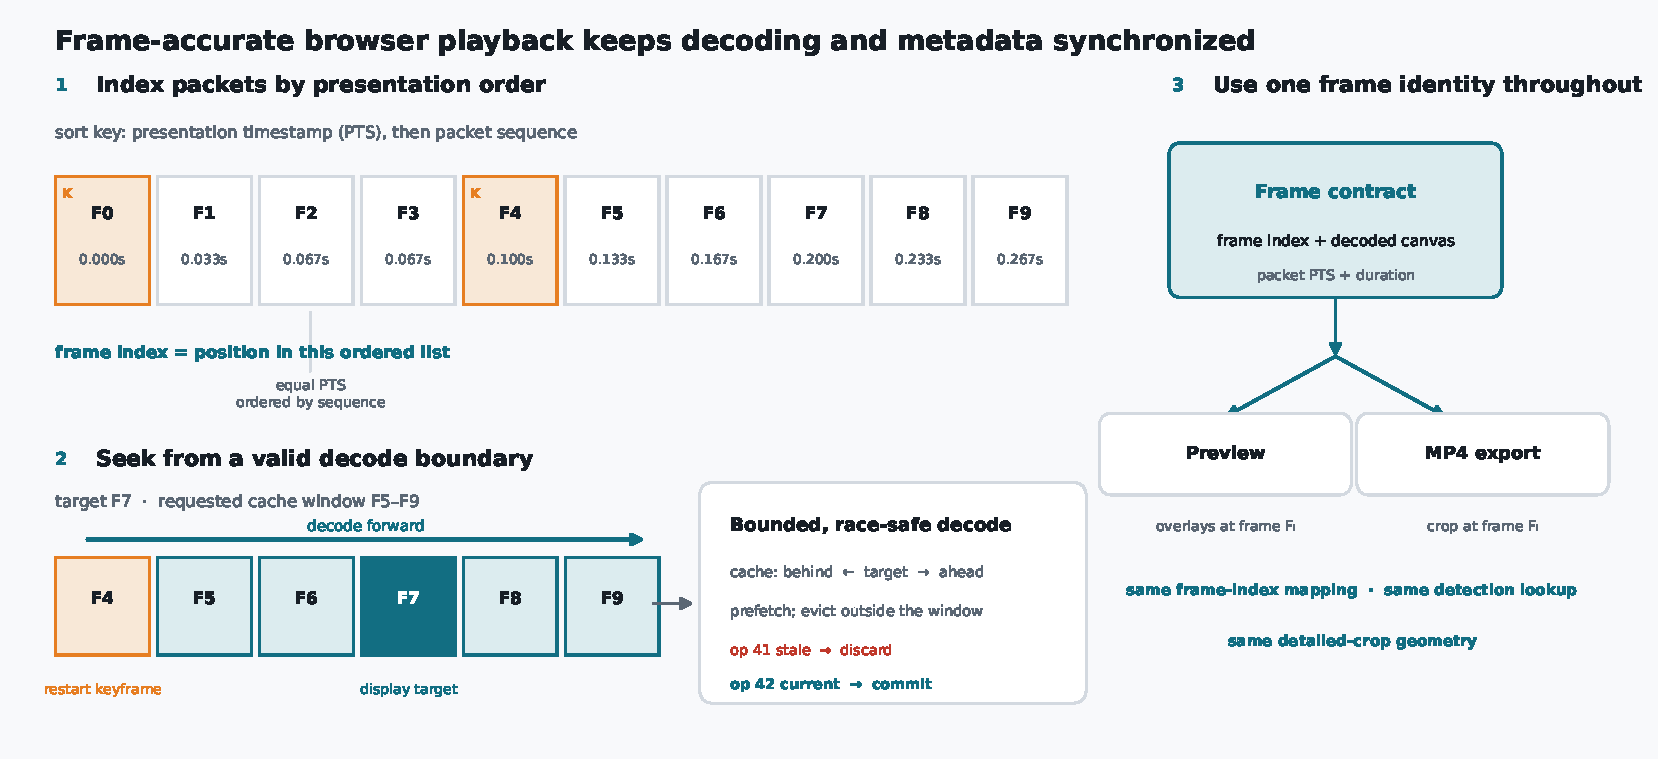
\includegraphics[width=\linewidth]{player-frame-accurate-playback.pdf}
  \caption{Preview and export decode independently but identify frame $i$ by the same
  ordered-packet index. Preview seeks from a preceding keyframe; export advances its
  own decoder and can resynchronize by timestamp. Both use the index for track lookup,
  while only focused rendering shares the pose-anchor crop function.}
  \label{fig:player-frame-contract}
\end{figure}

\section{Conclusion}
\label{sec:conclusion}

We presented an offline system that turns long-shot windsurfing video into stable,
rider-relative trajectories.  Its design follows the structure of the problem:
masked camera-motion estimation handles large pans, conservative local association
protects tracklet purity, sail-specific appearance and four-dimensional motion score
longer continuations, a global integer program uses complete-video context, and two
rig landmarks control the final virtual camera.

On 21 manually reconstructed development videos, the association subsystem improves
pairwise F1 and greatly reduces fragmentation relative to the evaluated OC-SORT and
BoT-SORT configurations.  The staged revision also shows why implementation details
matter: activating the intended foreground mask, aggregating appearance over whole
fragments, retaining box-size evidence, and vetoing implausible links collectively
reduce contaminated tracks from 20 to nine.  The remaining crossing errors and the
in-sample protocol preclude a claim of perfect or general-purpose tracking.  The
contribution is instead a reproducible account of how domain structure, offline
inference, and an explicit failure cost can make an otherwise ordinary detection
model useful in a demanding video-analysis system.


\begin{thebibliography}{9}
\bibitem{ocsort}
J. Cao, J. Pang, X. Weng, R. Khirodkar, and K. Kitani,
``Observation-Centric SORT: Rethinking SORT for Robust Multi-Object Tracking,''
\emph{CVPR}, 2023.

\bibitem{botsort}
N. Aharon, R. Orfaig, and B.-Z. Bobrovsky,
``BoT-SORT: Robust Associations Multi-Pedestrian Tracking,''
\emph{arXiv:2206.14651}, 2022.

\bibitem{webcodecs}
W3C Media Working Group,
``WebCodecs,'' W3C Working Draft.
\url{https://www.w3.org/TR/webcodecs/}
\end{thebibliography}

\end{document}
